% !Mode:: "TeX:UTF-8"
%% This is file `mcmthesis-demo.tex',
%% generated with the docstrip utility.
%%
%% The original source files were:
%%
%% mcmthesis.dtx  (with options: `demo')
\newcommand{\upcite}[1]{\textsuperscript{\textsuperscript{\cite{#1}}}}
\documentclass{mcmthesis}
\mcmsetup{
		CTeX = false,
        tcn = 69377,
        problem = E,
        sheet = true, 
        titleinsheet = true, 
        keywordsinsheet = true,
        titlepage = true, 
        abstract = true
}
\usepackage{palatino}
\usepackage{lipsum}
\usepackage{booktabs}
\usepackage{tabu}%%table
\usepackage{colortbl}
\usepackage{indentfirst}%%suojin
%% picture package-------------------
\usepackage{geometry}%页面设置  
\usepackage{graphics}%图片设置  
\usepackage{caption}%注释设置  
\usepackage{graphicx}
\usepackage{subfigure}
%%-------------------------

\title{Water Supply and demand model}
\date{\today}

 %正文摘要和控制页摘要名字修改
\def\abstractname{Abstract}
\def\sheetsummaryname{Summary}

\begin{document}

 %控制页摘要内容
\begin{sheetsummary}

\par In this paper, a model is established to evaluate a region’s ability to supply water. The model calculates the demand and supply of water resources in a region, and then compiles them to obtain the index $I_{SD}$, a positive value. How large the index indicates the level of the scarcity of water resources. As for demand, the use of water can be categorized into four classes: industrial use, agricultural use, domestic use and ecological use. In terms of supply, we define it as a combination of surface water, groundwater and other water. Others may refer to the increase in the amount of water due to technology advances, or the decrease as a result of pollution.
\par Then we select Beijing, an extremely water-scarce city, and analyze it through the data from the National Bureau of Statistics (NBS) from 2004 to 2015. Then, we analyze the trend of the consumption of agricultural water, industrial water, domestic water and ecological water. Polynomial fitting and gray prediction are used to forecast the annual demand and supply of water in Beijing in the next 15 years. By comparing the precision of the two methods, we select the one with higher prediction precision. And we discuss the advantages and disadvantages of the model.
\par We then provide a plan to mitigate water shortage in selected areas. We devise our plan by adjusting our Model Index $I_{SD}$. Specifically, we should consider both factors that affect the size of the index. Therefore, we can either increase the water supply or reduce the demand of water to ease water shortage. The detailed plan includes increasing water tariffs, increasing water recycling, adopting large-area drip irrigation in agriculture, increasing education to raise water-saving awareness, controlling population, and South-to-North Water Transfer Project.
\par Then we proceed with the rationale and rationality of the proposed scheme. We discuss how the price of water will affect the demand for water and achieve conclusions from recycled water and agricultural drip irrigation. We also analyze the short-term influence of education to alleviate water shortage. Nevertheless, inter-basin water transfer may lead to ecological damage, resulting in rising negative effects of water shortage.
\par Finally, we improve our model. We subdivide the $I_{SD}$ index that is less than 1 into four types: extremely scarcity, scarcity, stress and Borderline adequate.



\end{sheetsummary}

 %正文摘要内容
\begin{abstract}
\par In this paper, a model is established to evaluate a region’s ability to supply water. The model calculates the demand and supply of water resources in a region, and then compiles them to obtain the index $I_{SD}$, a positive value. How large the index indicates the level of the scarcity of water resources. As for demand, the use of water can be categorized into four classes: industrial use, agricultural use, domestic use and ecological use. In terms of supply, we define it as a combination of surface water, groundwater and other water. Others may refer to the increase in the amount of water due to technology advances, or the decrease as a result of pollution.
\par Then we select Beijing, an extremely water-scarce city, and analyze it through the data from the National Bureau of Statistics (NBS) from 2004 to 2015. Then, we analyze the trend of the consumption of agricultural water, industrial water, domestic water and ecological water. Polynomial fitting and gray prediction are used to forecast the annual demand and supply of water in Beijing in the next 15 years. By comparing the precision of the two methods, we select the one with higher prediction precision. And we discuss the advantages and disadvantages of the model.
\par We then provide a plan to mitigate water shortage in selected areas. We devise our plan by adjusting our Model Index $I_{SD}$. Specifically, we should consider both factors that affect the size of the index. Therefore, we can either increase the water supply or reduce the demand of water to ease water shortage. The detailed plan includes increasing water tariffs, increasing water recycling, adopting large-area drip irrigation in agriculture, increasing education to raise water-saving awareness, controlling population, and South-to-North Water Transfer Project.
\par Then we proceed with the rationale and rationality of the proposed scheme. We discuss how the price of water will affect the demand for water and achieve conclusions from recycled water and agricultural drip irrigation. We also analyze the short-term influence of education to alleviate water shortage. Nevertheless, inter-basin water transfer may lead to ecological damage, resulting in rising negative effects of water shortage.
\par Finally, we improve our model. We subdivide the $I_{SD}$ index that is less than 1 into four types: extremely scarcity, scarcity, stress and Borderline adequate.


\end{abstract}

 %关键词
\begin{keywords}
Supply and Demand of Water; GM(1,1); Fitting; Multi-factors Analysis  
\end{keywords}

\maketitle
 % Generate the Table of Contents, if it's needed.
\tableofcontents
\newpage


%%----------------------------------------------------------------------------------
\section{Introduction}
\subsection{Background} 
\begin{figure}[h]
\small
\centering
\includegraphics[width=14cm]{WSI_world.jpg}
\caption{UN Water Scarcity Map} \label{fig:UN water scarcity map}
\end{figure}
\par As the source of life, water is precious and indispensable to human beings. However, the amount of water available can hardly satisfy our need. There is a huge number of water on the earth, but the water that can be directly used in production and life seems pitiful. First of all, sea water contains salt so it is bitter. We cannot drink it or use it for industry without treatment. Secondly, the amount of fresh water resources accounts for only $2.5\%$ of the total amount of water. And in the very little water volume, more than $70\%$ is frozen in the Antarctic and the Arctic ice cap, which is difficult for people to use.
\par At present, about 1 billion 500 million people in more than 80 countries around the world are facing water shortages (showed in the figure 1)\upcite{14}. Thus it’s significant to know the supply and demand of clean water and how to predict the future water scarcity and design an intervention plan. For example, in Beijing, the northern city in China, it shows that per capita water resources in 2011 is 134 cubic meters through China water conservancy statistics. Compared with the UN statistics, Beijing suffers from severe water shortage. Its per capita water resource is about to be dropped to 100 cubic meters, which is less than $1/20$ of that in China, and less than $1/80$ of that in the world.
\subsection{Our work} 
\par There have been many methods developed to analyze the problem of water scarcity. The analysis of regression is used to predict the future supply and demand of water according to the historical data. And analytic hierarchy process is used to design an intervention plan. $SD$ model\upcite{1} is an analysis on the feedback information, the dynamic behavior between function and space. 

\par In our article, we use the Multi-factors model to analyze the supply and demand of water resources.  And we use the improved $GM(1,1)$ model\upcite{2} to predict. This grey prediction model needs less data, but can provide not only more accurate prediction, but more simple and convenient calculation when sample distribution is not regular.
\section{Symbol Description}
\par In the section, we use some symbols for constructing the model as follows.
\begin{center}
\begin{tabular}{cc}
\toprule 
Symbol & Description\\
\midrule
$I_SD$ & Index to measure the ability to provide clean water to meet the needs \\
$W_S$ & The amount of water that a region supply\\
$W_D$ & The amount of water that a region demand\\
$MRE$ & Mean relative error of predict model\\
$R$ & Relevancy of predict model\\
\bottomrule
\end{tabular}
\end{center}




%%-----------------------------------------------------------------------------------
\section{Analysis of the Problem}
\par The International Clean water Movement (ICM) wants our team to build a model to help them solve the world’s water problems by improving access to clean, fresh water. 
\begin{itemize}
	\item Develop a model that provides a measure of the ability of a region to provide clean water to meet the needs of its population. And take the dynamic nature of the factors that affect both supply and demand into consideration.
	\item Choose a region (we choose Beijing in the UN water scarcity map where water is heavily overloaded) and explain the reason why water scarcity situation there is heavy at present comprehensively.
	\item Make some predictions in 15 years.
	\item Come up with an intervention plan and assess the effect of it. And we need to think about the impact and the overall strengths and weaknesses of the plan in this larger context.
	\item When designing our model, we should take interdisciplinary elements into consideration. And it’s necessary to consider our plan’s reliability.
	\item By comparing the water scarcity under our intervention with that under no intervention,  improving our plan and discuss the strengths and weaknesses.
\end{itemize}


%%________________________________________________________________
\section{Key Points of Our Model}
\subsection{Assumptions}
\par Some elements are unpredictable, which we do not include in our model. So our model requires the following assumptions:
\begin{itemize}
	\item No major natural disasters happen.
	\item No major policy reforms take place.
	\item The economy of the region develops steadily.
	\item Population growth stays moderate.
\end{itemize}
\par What need to be mentioned here is the things above only happen at an extreme small possibility. So they don’t affect our model’s justifiability.

\subsection{Approach}
\par When building our model, we mainly adopt three approaches.
 
\subsubsection{Multi-factors analysis}
\par To evaluate the ability of a region to offer clean water, we need consider supply as well as demand. We apply industrial use, agricultural use, domestic use and ecological use to describe demand, and define supply as a combination of surface water, groundwater and other water. This is the first level of our Multi-factors analysis.
\par However, if we don’t have the data above, we can also estimate it, which serves as the second level of our Multi-factors analysis. For example, we can utilize industrial production to compute the amount of industrial water\upcite{3}. We can use the area of cultivated land and grain yield to assess the amount of agricultural water\upcite{4}. We can also use gross domestic product per capita to estimate domestic water\upcite{5}.

\textbf{We apply the next two approaches for prediction. In a specific situation, we compare them and choose the more effective one. }

\subsubsection{GM(1,1) model}
\par Based on the data we have, we employ the model for prediction. The model prevails compared with other models when devoid of statistics. We only have data in several years to deliver reliable forecast. So it can suit our situation quite well.

\subsubsection{Fitting model}
\par We fit some values of the dependent variables as well as the independent variable. We determine the values of the coefficients when achieving the minimal set difference (least squares sense).


\section{Calculating the Model}
\subsection{Basic Model}
\par When designing our model, we should take interdisciplinary elements into account. To evaluate the ability of a region to offer clean water, we need consider supply as well as demand. As for demand, the use of water can be categorized into four classes: industrial use, agricultural use, domestic use and ecological use. In terms of supply, we define it as a combination of surface water, groundwater and other water. Others may refer to the increase in the amount of water due to technology advances, or the decrease as a result of pollution. In the process, the scale of population, the state of economy and the development of technology all have a significant influence on both supply and demand, giving rise to their dynamic nature.

\begin{figure}[h]
\small
\centering
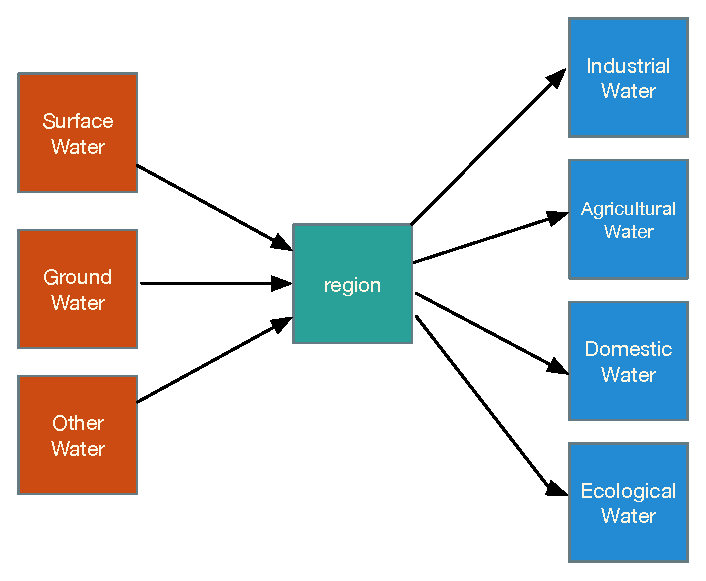
\includegraphics[width=8cm]{waterSupplyDemand.eps}
\caption{Water Supply and Demand In a Region} \label{fig:Water Supply and Demand In a Region}
\end{figure}

\par Only including major factors, we give the following calculation formulas.
\begin{equation}
	I_{SD} = \frac{W_S}{W_D}
\end{equation}
\par We define the index to measure the ability to provide clean water to meet the needs as $I_{SD}$. 
\begin{equation}
	W_S = W_{Ss} + W_{Sg} - W_{Sr} + W_{So}
\end{equation}
\par In formula(2) $W_{Ss}$ is the the amount of surface water supply; $W_{Sg}$ is the the amount of groundwater supply; $W_{Sr}$ is the the amount of repeatedly calculated water supply; $W_{So}$ is the other sources of water supply.
\begin{equation}
	W_D = W_{Di} + W_{Da} + W_{Dd} + W_{De}
\end{equation}
\par In formula(3) $W_{Di}$ is the the amount of industrial water demand; $W_{Da}$ is the the amount of agricultural water demand; $W_{Dd}$ is the the amount of domestic water demand; $W_{De}$ is the the amount of ecological water demand.
\par If a region is pretty capable to supply water, then $I_{SD}$ will be a number greater than 1. The larger the number is, the higher its ability to supply water is. Nevertheless, the region lacks water when $I_{SD}$ is a number smaller than 1. 
\par To know the ability of a region to provide clean water, we just need to fit in the current values of these parameters. Even though we don’t know the exact values of them in the future, we can predict them with certain methods. In our model, we can use \emph{fitting} or \emph{GM(1,1)} model.

\subsection{Model Application}

\begin{figure}[h]
\small
\centering
\includegraphics[width=10cm]{whybeijing.png}
\caption{The Water Resource Shortage in China} \label{fig:The Water Resource Shortage in China}
\end{figure}


\par In the UN water scarcity map where water is heavily overloaded, we choose Beijing.
We want to obtain $I_{SD}$ of Beijing to measure its ability of to provide clean water to meet the needs. To determine the value of $W_S$ and $W_D$, we want to try the \emph{fitting} and \emph{GM(1,1)} on this problem at first, and choose the better one to apply to our model.
\par We have values of these parameters above in Beijing from 2004 to 2015. Based on the data, we can apply the methods and calculate the mean relative error separately.
 
\subsubsection{The Two Algorithms: Fitting and GM(1,1)}
\textbf{Fitting} 
\par In fitting model, we fit some values of the dependent variables as well as the independent variable, and obtain the values of the coefficients when achieving the minimal set difference (least squares sense. Now we need to find out the relationship between $W_D$(annual water demand) with the year through the data of 12 years (2004-2015) given by the National Bureau of Statistics. Based on this, we can predict the water consumption over the next 15 years. Similarly, we can find the relationship between $W_S$(annual water supply) with the year through the given data.

\begin{figure}[htbp]  
\begin{minipage}[t]{0.5\textwidth}
\centering  
\includegraphics[width=\linewidth]{water_use_4_line.png}  
\caption{Water Use with Linear Fit} 
\end{minipage}
\begin{minipage}[t]{0.5\textwidth}  
\centering  
\includegraphics[width=\linewidth]{water_use_4.png}  
\caption{Water Use with Polynomial Fit}  
\end{minipage}  
\end{figure} 

\emph{Linear Fit}
\par Given discrete data where $X_k$ is the value of the independent variable $X$ (scalar or vector, ie, one or more variables); $Y_k$ is the corresponding value of the dependent variable $Y$ (scalar), if the function to be determined is linear, it is called linear fit or linear regression (mainly in statistics).
\par Both water demand and water supply vary with the year. Generally, we Input the yearly independent variable $X_k$ as well as the corresponding annual water consumption or water demand $Y_k$, and use the least squares method to calculate the empirical regression formula.
\par The result showed in figure 4.

\emph{Polynomial Fit}
\par In fact, there is not necessary a linear relationship between variables, such as the relationship between drug concentration and time, disease efficacy and duration of treatment or toxic dose and lethality. Curve fitting is to select the appropriate curve type to fit the observed data, and use the fitting curve equation to analyze the relationship between two variables. 
\par In order to improve the accuracy of fitting, try polynomial fitting to observe whether the fitting accuracy is improved.
\par The result showed in figure 5.

\par The coefficient index of the two fitting method show in following table:

\begin{center}
	Coefficient Index of the Two Fitting Method\\
\begin{tabular}{lcccc}
\toprule 
 & Agricultural & Industrial & Domestic & Ecological \\
\midrule
Linear Fit & 0.93 & 0.7822 & 0.9433 & 0.9091 \\
Polynomial Fit & 0.9759 & 0.861 & 0.9482 & 0.9547\\
\bottomrule
\end{tabular}
\end{center}
\par Contrast the table data, we choose Polynomial fit.\\

\textbf{GM(1,1)}

\par The traditional GM (1,1) model is composed of a differential equation containing univariate.
\par Let $X^{(0)}=[x^{(0)}(1), x^{(0)}(2),\cdots ,x^{(0)}(n)]$ , $X^{(1)}=[x^{(1)}(1), x^{(1)}(2),\cdots ,x^{(1)}(n)]$ , $Z^{(1)}=[z^{(1)}(1), z^{(1)}(2),\cdots ,z^{(1)}(n)]$ , where $x^{(1)}(k) =  \sum\limits_{i=1}^k x^{(1)}(i)$ and $z^{(1)}(k) = \frac{x^{(0)}(k) + x^{(0)}(k+1)}{2}$ , then $x^{(0)}(k) + a z^{(1)}(k) = b$ is called the GM(1,1) model. The parameter $a$ is called the development coefficient, and the parameters $b$ is called the grey action quantity.
 
Then, we can get the time responded function of GM(1,1) model.
\begin{equation}
	\hat{x}^{(1)}(k+1) = (x^{(0)}(1) - \frac{b}{a})e^{-a k} + \frac{b}{a} \qquad k = 1, 2, \cdots, n
\end{equation}
and the restored function of $x^{(0)}(k + 1)$ can be given by

\begin{equation}
	\hat{x}^{(0)}(k+1) = (1 - e^a)(x^{(0)}(1) - \frac{b}{a})e^{-a k} \qquad k = 1, 2, \cdots, n
\end{equation}

\par In which, $\hat{x}^{(1)}(k)$ is the simulative value of  $x^{(1)}(k)$, and  $\hat{x}^{(0)}(k)$ is simulative value of $x^{(0)}(k)$

\par Without external interference, we know that the population and GDP was exponential growth. But this model will produce a continuously simulative deviation when simulating a homogeneous-exponent sequence. Because the unequal conversion between the discrete difference equation and continuous differential equation. So we learn from C.I.Chen\upcite{}. The Discrete GM(1,1) Model as follows:
\begin{equation}
	\hat{x}^{(1)}(k+1) = (x^{(0)}(1) - \frac{b}{a})(\frac{2 - a}{2 + a})^k+ \frac{b}{a} \qquad k = 1, 2, \cdots, n
\end{equation}
\begin{equation}
	\hat{x}^{(0)}(k+1) = (1 - \frac{2 + a}{2 - a})(x^{(0)}(1) - \frac{b}{a})(\frac{2 - a}{2 + a})^k \qquad k = 1, 2, \cdots, n
\end{equation}
\par Use least squares to solve $a$ and $b$. Put it into the prediction formula. We can get the predictive value $X^{(1)}$, and the analog value of $X^{(0)}$.\\

\textbf{evaluation criterion}
\par We use two values to reflect the prediction accuracy.

\begin{itemize}
	\item Mean Relative Error:
	\begin{equation}
		MRE = \frac{1}{n} \sum \limits_{k = 1}^n \frac{\mid x^{(0)}(k) - \hat{x}^{(0)}(k) \mid}{x^{(0)}(k)}
	\end{equation}
	\item Relevancy:
	\begin{equation}
		R = \frac{1}{n} \sum \limits_{k = 1}^n \frac{\min \{\mid x^{(0)}(k) - \hat{x}^{(0)}(k) \mid\} + l \times \max\{\mid x^{(0)}(k) - \hat{x}^{(0)}(k) \mid\}}{\mid x^{(0)}(k) - \hat{x}^{(0)}(k) \mid + l \times \max\{\mid x^{(0)}(k) - \hat{x}^{(0)}(k) \mid\}}
	\end{equation}
	\par Among formula, $l$ is resolution ratio, usually the value is $0.5$. It`s meaningful when $R \geq 0.6$.
\end{itemize}


\subsubsection{Implementation and Comparison between Polynomial Fit and GM(1,1)}
\par We use the existing data to create a chart showed figure 6. 
\par What is need to be particularly noted is that bad values should be eliminated to guarantee the method’s performance. From the National Bureau of Statistics data in 2008, 2012, 2014, water supply is particularly big in 2008 because of a large number of afforestation before the Olympic Games. In 2012, water supply is also large due to a huge flood. However, it experiences a sheer drop as a result of drought in 2014, the affected area of which covers 26.1 thousand hectares. In our assumptions, we do not take the impact of disasters into account, so we remove the data at 2008, 2012 and 2014 to make our model more effective. so we remove these bad values. 
\par Then we get a new figure 7.

\begin{figure}[htbp]  
\begin{minipage}[t]{0.5\textwidth}
\centering  
\includegraphics[width=\linewidth]{water_sd_bad.png}  
\caption{Supply and Demand Curve of Water in 2004-2015} 
\end{minipage}
\hspace{1ex}
\begin{minipage}[t]{0.5\textwidth}  
\centering  
\includegraphics[width=\linewidth]{water_sd_good.png}  
\caption{Supply and Demand Curve of Water in 2004-2015 Without Bad Value}  
\end{minipage}  
\end{figure} 

\par We use the two methods to predict the data of Beijing`s water supply and demand\upcite{15}. And get the following table.

\begin{center}

	The Data and Simulate Table of $W_D$ and $W_S$ (unit:$1\times10^9m^3$) 
	
\begin{tabular}{l|cccccccccc}
\toprule
 & 2004 & 2005 & 2006 & 2007 & 2009 & 2010 & 2011 & 2013 & 2015 & 2030\\
\midrule
$W_D$ Data & 34.55 & 34.50 & 34.30 & 34.81	& 35.50 & 35.20 & 35.96 & 36.38 &	38.20 & \\
$W_D$ Simulate & 34.55 & 33.97 & 34.42 & 34.89 & 35.35 & 35.83 & 36.31 & 36.79 & 37.29 & 45.53\\
$W_S$ Data & 21.34 & 23.18 & 22.07 & 23.81 & 21.84 & 23.10 & 26.81 & 24.81 & 26.80 & \\
$W_S$ Simulate & 21.34 & 22.01 & 22.56 & 23.13 & 23.71 & 24.31 & 24.92 & 	25.55 & 26.20 & 38.04\\
\bottomrule
\end{tabular}


\end{center}

\par We calculated the MRE values of the two methods from the predicted data showed in the following table.
\begin{center}
	Algorithm Comparison
\begin{tabular}{l|cc}
\toprule 
Predict Method & $W_S$ Predict $MRE$ &  $W_D$ Predict $MRE$\\
\midrule
GM(1,1) & 0.0402698929930414 & 0.0068299550666618\\
Fitting & 0.0392193960593265 & 0.00978166931838276\\
\bottomrule
\end{tabular}
\end{center}

\par By compare the MRE value of two methods, we choose to use the GM(1,1) model.




\subsubsection{the model results and analysis}
\par To begin with, it is essential to know about climate and geology of Beijing to identify their impact on water resources. Beijing is located in the northwest corner of the Great Plains, $115^o25'$ E ~ $117^o30'$E, $39^o28'$N ~ $41^o05'$N, with a total area of about $1.68\times10^{10}m^3$. Beijing is located in the transition zone between mountain($62\%$) and plain($38\%$). Northeast , North and West mountains stand, and the southeast is a gentle slope to the southeast of the plain, forming a special mountain to the sea, commonly known as "Beijing Bay" showed in figure 8.

\begin{figure}[h]
\small
\centering
\includegraphics[width=8cm]{beijing.jpg}
\caption{China Water resource shortages} \label{fig:China Water resource shortages}
\end{figure}

\par Beijing climate belongs to warm temperate semi-humid semi-arid monsoon climate. In spring, the temperature rises rapidly and the change in temperature of the day is more significant; summer is hot and rainy; autumn is suitable for cold and warm, sunny and rainy; winter is cold and dry. And the rain and heat are suitable for a variety of crops But it is located in the intersection of cold and warm air, annual precipitation variability, the main meteorological disasters are drought, rain, wind, hail, cold and so on.
\par Precipitation is the main source of water supply for Beijing. Annual precipitation (1956-2002) is $594.4 (mm)$, equivalent to the amount of precipitation is 99.86 million($m^3$), of which $60\% -70\%$ evaporation loss, only a small part of the runoff and infiltration underground. While the average water resources in Beijing over the same period the total of 3.739 billion($m^3$). Up to 1956 years, 96.53 million($m^3$), at least in 2002 to 1.611 billion($m^3$). At present, Beijing's total annual water demand is 4.6 billion($m^3$), far more than the average annual water supply capacity. Therefore, the total amount of natural precipitation in Beijing is inadequate, in a state of water shortage.
\par Then, we want to know how scarce water is in Beijing. Because we don’t have data of 2016, we also assess it based on our model. In 2016, $I_{SD} = 0.709 < 1$, obviously, Beijing is lack of water.
\par The reasons why water is scarce in Beijing can be divided into two aspects, physical and economic ones. 

\begin{itemize}
	\item Physical scarcity
	
	\par It is closely related to the local environment. According to the collected data, the water resources per capita in Beijing from 2011 to 2015 are 124.01($m^3$), 95.15($m^3$), 118.59($m^3$), 193.24($m^3$),134.71($m^3$). The average is 133.14($m^3$). However, the water resources per capita in China from 2011 to 2015 are 2039.25($m^3$), 1998.64($m^3$), 2059.69($m^3$), 2186.05($m^3$), 1730.20($m^3$). The average is 2002.766($m^3$), $1/4$ of the world water resources per capita, but 15 times of that in Beijing.
	\item Economic scarcity
	
	\par we cannot ignore the social factors. The first is the huge population, 20 million citizens. The second is people’s awareness of saving water. Last, the current environmental pollution and imperfect sewerage system also lead to the severe situation.
\end{itemize}


\section{Model Application in Prediction}

\begin{figure}[htbp]  
\begin{minipage}[t]{0.5\textwidth}
\centering  
\includegraphics[width=\linewidth]{W_S_pre.png}  
\caption{$W_S$ in 2004-2030 without 2008,2012,2014} 
\end{minipage}
\hspace{1ex}
\begin{minipage}[t]{0.5\textwidth}  
\centering  
\includegraphics[width=\linewidth]{W_D_pre.png}  
\caption{$W_D$ in 2004-2030 without 2008,2012,2014}  
\end{minipage}  
\end{figure} 

\begin{figure}[h]
\small
\centering
\includegraphics[width=12cm]{index_good.png}
\caption{$I_{SD}$ in 2004-2030 without 2008,2012,2014} \label{fig:$I_{SD}$ in 2004-2030}
\end{figure}

\par According to the figure 9-11, we can easily detect a trend that ISD is slowly increasing, which means Beijing’s ability to supply clean water is improving. But $I_{SD}$ doesn’t exceed 1, so the water supply still does not meet the demand. So citizens in Beijing need to save water. For example, they can reuse water in the daily life. Furthermore, we know although $W_D$ is rising, $W_S$ is increasing at a faster speed. 

\begin{figure}[h]
\small
\centering
\includegraphics[width=12cm]{water_and_tree.png}
\caption{$W_S$ and Forestry land area in 2004-2015} \label{fig:$W_S$ and Forestry}
\end{figure}

\par We can see from figure 12. Beijing dedicates a lot to afforestation. The improvement in environment contributes much to the growth in $W_S$. Especially, we can see, in 2008, there is a steep rise in forestry land area. Simultaneously, $W_S$ is at its peak in these years.





\newpage
\section{Intervention Plan Based on Our Model}

\par Beijing is in the arid regions of northern China. The shortage of water resources, combined with environmental degradation and increasing population, has aggravated the situation of water resources.

\par The plan to alleviate the water crisis is very necessary. Then, we will improve the awareness of water crisis and water-saving, improve the water use efficiency of industry, agriculture and life, and strengthen the utilization of  the rainwater. Vigorously promoting agricultural water-saving measures are to strengthen the groundwater reserves and establish a sound water resources management system.

\par Alleviating the problem of water shortage in Beijing can mainly reduce the demand for water resources or increase the supply of water resources, so as to alleviating the problem of water shortage.

\begin{itemize}
	\item Strategy 1: To Enhance Water Prices
	
	\par The price increase will be used to influence the demand for water directly, the demand for industrial and agricultural water will be reduced significantly, and the impact on domestic water will be significant. Therefore, the price will be used to stimulate the user to reduce water use. In the economic market ,affect the supply curve of the movement, thereby reducing the water from the rivers and lakes to achieve the supply and demand are reduced to a new equilibrium.
	\begin{figure}[h]
	\small
	\centering
	\includegraphics[width=12cm]{sd.png}
	\caption{Supply and Demand Curve of Water} \label{fig:Water Supply and Demand}
	\end{figure}
	
	\item Strategy 2: Increase The Use of Rainwater Flooding and Sewage
	
	\par It is an important way to solve the problem of water resources in Beijing by attaching great importance to the utilization of rainwater flood and utilization of sewage. A large number of surveys and researches by the Beijing Department of Geology and Mineral Resources also shows that there is a large area of ​​about 400$km^2$ sandy gravel permeable layer in the western suburbs of Beijing, with good infiltration conditions, is the establishment of underground reservoirs, the ideal place for artificial storage; The Guan ting Gorge, with an area of ​​1600$km^2$, is a heavy rainstorm area in the west of Beijing with an annual runoff of 0.4-2.5 billion $m^3$. Through the new west suburb 26.2$km^2$ gravel pit flood storage and reclamation project, the average annual rechargeable water is 2.2 million $m^3$. 
	
	\par It will play a positive role in relieving the groundwater resource tensions in the western suburbs of Beijing. On the other hand, full use of green land infiltration is another effective way to utilize rainwater flooding resources, which not only can reduce the irrigation water quantity of green land, but also can reduce the burden of drainage channels\upcite{9,10} improve the development and utilization of water, to achieve the use of sewage, but also to solve the shortage of water resources. Beijing should be built in a large number of water facilities, the facilities to bathing, washing and other domestic sewage as water, after treatment to meet the water quality standard, you can be back for flushing, car washing, greening, etc.
	\item Strategy 3: Development of Agricultural Drip Irrigation Water-saving Technology
	
	\par The purpose of water-saving agriculture is not only to make the most effective use of valuable water resources, but also to make the limited water resources to promote agricultural production, improve the quality of agricultural products, improve land resources, agricultural production and living environment continues to improve. In 2006, Beijing's agricultural water consumption accounted for nearly $40\%$ of the total water consumption, while the phenomenon of irrigation water waste is still common. Some areas are still  using "soil drainage, flood irrigation" approach, half of irrigation water in the water .The proportion of not more than $20\%$, most of the water is consumed by evaporation\upcite{13}. In addition, the water content of underground water, The utilization coefficient of agricultural irrigation water in Beijing is $0.3 \sim 0.4$, and the production efficiency of grain water is about $1 kg/m^3$. The utilization coefficient of irrigation water in developed countries is generally around 0.8. The water-saving irrigation project in Beijing still has great potential. The actual situation in Beijing reduce agricultural ineffective evaporation and improve agricultural water efficiency.
	\item Strategy 4: Reduces the Population Growth Rate in Beijing
	
	\par The population has a significant impact on the demand for water resources. As the graph below illustrates, as the population grows, the average amount of water consumed per person per year increases, the demand for water increases, and the supply of water increases.
	
 	\par In addition to the natural growth rate, the population of Beijing should also consider the net migration rate. If the population growth rate can be limited, the demand for water will be directly reduced (showed in figure 14).
	
	\par Additionally, Slowing Population Growth The 1994 United Nations International Conference on Population and Development (ICPD) provided an opportunity for countries to examine their population challenges and discuss possible solutions for achieving socially equitable, sustainable development for each country. The ICPD Program of Action focuses on human development, providing a framework for slowing population growth and improving people's lives. It calls for a wide range of investments to improve health, education, and rights particularly for women and girls and to provide reproductive health information and services to help people to achieve their desired family size. 
	
		\begin{figure}[h]
		\small
		\centering
		\includegraphics[width=12cm]{people.png}
		\caption{Population Growth With $W_S$ and $W_D$} \label{fig:Population Growth With $W_S$ and $W_D$}
		\end{figure}
		
	\item Strategy 5: Inter-basin Water Transfer
		
	\par "South-to-North Water Transfer Project" is a strategic project of the People's Republic of China. Referring to the Yangtze River Basin water resources from its upstream, midstream, downstream, combined with the characteristics of China's territory, the eastern, central and western part of the transfer line sent to the North China , the Huai River Plain and the Northwest region of water shortages. That midline Planning $70\%$ of the water is from the Han River Basin, Shaanxi Han Zhong, An Kang, and Shang Luo area, converge to the Dan Jiang Kou Reservoir, Dan Jiang Kou Dam increased by the Dan Jiang Kou reservoir after the transfer of water, from Henan Nanyang water, Henan He Nan southwest Tang Bai He Yangtze River Basin and the Huai River watershed Fang Cheng Pass, after the western edge of the Huang Huai Hai Plain, west of Zhengzhou in the mouth through the Yellow River, continue along the west side of the Beijing-Guangzhou Railway, the basic gravity to the end of Beijing.
	
	\par Beijing could divert water from the midline project, thereby increasing the supply of water in the water supply and increasing the supply of water to alleviate water shortages in Beijing.
\end{itemize}

\section{Evaluation of the Intervention Plan}
\par We are going to analyze whether the intervention we designed with our model will have the desired effects in the future.
\begin{itemize}
	\item Strategy 1: To Enhance Water Prices
	
	\par As is depicted in the picture, the $S_1$ and D curves in figure 13 depict the initial equilibrium of the market. As the price of water rises, new demand for water is reduced and water supply is increased, leading to new Demand $Q_{2D}$, so the supply curve shifts to the left, to a new equilibrium. We can reduce water consumption, so that we can reduce the $I_{SD}$.
	\item Strategy 2: Increase The Use of Rainwater Flooding and Sewage
	
	\par At present, rainwater flooding in Beijing has made initial progress, the relevant departments have increased the construction of rainwater flooding facilities. Beijing has been built Tian xiu Park, Double Purple District, Beijing Normal University, Beijing Hydropower School and more than 50 rainwater utilization demonstration project. Improve the level of rainwater use. It is predicted that in the plain area of Beijing rainwater utilization engineering system and floodgate recharge will increase the amount of groundwater recharge more than 100 million $m^3$. The rainwater flooding utilization in the urban area can reach 1.0-1.5 Billion $m^3$\upcite{11} and the utilization of water in 2007 is 480 million $m^3$, the equivalent of Miyun Reservoir in the water supply rate of $50\%$ utilization. We can reduce water consumption and increase the water supply, so that we can reduce the $I_{SD}$. 
	\item Strategy 3: Development of Agricultural Drip Irrigation Water-saving Technology
	
	\par The utilization of water is high up to $90\%$,higher than the diffuse irrigation water conservation $50\% \sim 60\%$. We can reduce water consumption in agriculture, so that we can reduce the $I_{SD}$. 
	\item Strategy 4: Reduces the Population Growth Rate in Beijing
	
	\par More people need more water. There are a number of factors that influence the population. The reduction in fertility through women's education is long-term and not significant in the short term in the above-mentioned prevention and control measures, so it is more difficult to reduce the natural rate of increase to get faster results. While it is more difficult to control the growth of its population in relation to the population moving into it. Therefore, a comprehensive analysis, by reducing the population to reduce the demand for water is a long process.

	\item Strategy 5: Inter-basin Water Transfer
	
	\par Transfer Project has been begun in 2010 after the full range of water. Beijing will be the annual water supply $1 \times 10^9 m^3$. The water supply including urban areas, Daxing, Tongzhou ,Fangshan, Mentougou and other areas, solves the problem of water shortage in the southwest of Beijing. And the existing seven urban underground water plant and self-control wells control the mining or stop mining to solve the city center Regional over-exploitation of groundwater, urban environmental water and other issues, and conserve and restore groundwater, to improve the purpose of urban water supply security. It may increase the $I_{SD}$.
	
	\par However, it may cause some bad impact by South-to-North Water Transfer Project on Beijing's Geological Environment.
	
	\par According to the present situation of water demand and surface water supply in Beijing, the South-North Water Transfer Project and the local surface water can not meet the urban water demand. It needs to use part of the groundwater to meet the water demand, and the local water resources can’t be conserved through the urban groundwater. 
\end{itemize}




\section{The Improvement of Our Model}
\textbf{Index Hierarchy}

		\begin{figure}[h]
		\small
		\centering
		\includegraphics[width=12cm]{Chinawater.png}
		\caption{Population Growth With $W_S$ and $W_D$} \label{fig:Population Growth With $W_S$ and $W_D$}
		\end{figure}
		
\par As described in the table, we will divided the $I_{SD} < 1$ into 4 parts. When the index is below 0.25, we define it as Extreme Scarcity. When the index is in the range of 0.25 to 0.5, we define it as Scarcity When the index is in the range of 0.5 to 0.75, we define it as Stress. When the index is in the range of 0.75 to 1, we define it as Borderline adequate. Additionally, when the index is above 1, we define it Adequate.
	\begin{center}
	The Value of Water Shortage State\\
	\begin{tabular}{lccccc}
	\toprule 
	 & Extreme scarcity & Scarcity & Stress & Borderline adequate & Adequate\\
	\midrule
	$I_{SD}$ & 0.25$\leq$ & 0.25$\sim$0.5 & 0.5$\sim$0.75 & 0.75$\sim$1 & $\geq$ 1 \\
	\bottomrule
	\end{tabular}
	\end{center}



\section{Strengths and weaknesses}


\subsection{Strengths}
\begin{itemize}
\item Our index $I_{SD}$ is an accurate indicator of evaluating the ability of a region to supply clean water.
\item Our model can make predictions with small set of data.
\item We have two methods for prediction. Furthermore, we can choose the appropriate one according to a given situation.
\item Our model is simple and easy to operate.
\end{itemize}

\subsection{weaknesses}
\begin{itemize}
\item Our model will deviate from the reality when any of the following situations occur:
\item Major natural disasters happen.
\item Major policy reforms take place.
\item The economy of the region remains unstable.
\item Population changes violently.
\end{itemize}
%%--------------------------------------------------------
%%reference-----------------------------------------------
\begin{thebibliography}{99}
\bibitem{1} Zhang, Z. W., et al. "Study on water resources carrying capacity based on system dynamics (SD) model in Hebei province." China Rural Water and Hydropower 3 (2008): 20-23.
\bibitem{2}Zhou, Wei, and Jian-Min He. "Generalized GM (1, 1) model and its application in forecasting of fuel production." Applied Mathematical Modelling 37.9 (2013): 6234-6243.
\bibitem{3} ZHAI, Chun-jian, Hong-wei ZHANG, and Liang WANG. "Application of industrial production function method to prediction of urban industry water consumption." Journal of Tianjin Polytechnic University 5 (2009): 023.
\bibitem{4}Jing, Huang, et al. "Agricultural water consumption trend and its influence factors in Beijing over the past 20 years." Journal of China Agricultural University 14.5 (2009): 103-108.
\bibitem{5} Qi-ting, Z. U. O. "Interval S-model for forecasting per capita domestic water consumption [J]." Journal of Hydraulic Engineering 3 (2008): 015.
\bibitem{6} Li, L., and Q. Fu. "Study on the city water resources capacity model with partial least-squares regression." Advances in Water Science 16.6 (2005): 822.
\bibitem{7}Wu, Chun-yan, Chun-yi Xuan, and Zhong-li Liu. "Study on the influences and countermeasures of climatic change to the sustainable development of water resources in Beijing Area." Chinese J Agrometeorol 30.S2 (2009): 200-204.
\bibitem{8} C.I. Chen, H.L. Chen, S.P. Chen, Forecasting of foreign exchange rates of Taiwan’s major trading partners by novel nonlinear Grey Bernoulli model NGBM
(1,1), Commun. Nonlinear Sci. Numer. Simul. 12 (6) (2008) 1194–1204.
\bibitem{9} Wu, P. L., and W. Zhang. "Water crisis and sustainable water resource utilization in Beijing." Journal of Liaoning Technical University (2005). 
\bibitem{10} Guo, Honglei, and X. Liu. "On Design and Construction of Rainwater Utilization Project." Municipal Engineering Technology (2010). 
\bibitem{11} Qiang, Zhu, and L. I. Yuan-Hong. "On the theoretical and practical significant of rainwater harvesting and utilization." Journal of Hydraulic Engineering (2004).
\bibitem{12}Guo qing, W. U. "Study on ecological safety and its evaluation of regional agricultural sustainable development." Journal of Natural Resources(2001).
\bibitem{13} Wang, H., C. Liu, and G. Mao. "Negative effects of water scarcity on agriculture in Beijing and countermeasures." Journal of Natural Resources 19.2(2004):160-169.
\bibitem{14}\url{http://www.unep.org/}
\bibitem{15}\url{http://data.stats.gov.cn/}
\bibitem{16}\url{http://worldwater.org/}
\bibitem{17}\url{http://www.prb.org/Publications/Reports/2002/}

\end{thebibliography}
%%---------------------------------------------------------

\end{document}

%% End of file `mcmthesis-demo.tex'.
